% Created 2013-12-20 金 04:52
\documentclass[12pt]{jsarticle}
\usepackage[dvipdfmx]{graphicx}
\usepackage{comment}
%\usepackage{setspace}
%%\date{\today}
%\title{}
\textheight = 25truecm
\textwidth = 18truecm
\topmargin = -1.5truecm
\oddsidemargin = -1truecm
\evensidemargin = -1truecm
\marginparwidth = -1truecm
\def\theenumii{\Alph{enumii}}
\def\theenumiii{\alph{enumiii}}
\def\labelenumi{(\theenumi)}
\def\labelenumiii{(\theenumiii)}
%\setstretch{0.9}
\begin{document}

%\maketitle
%\tableofcontents

\begin{center}
%%%%%%%%%%%%%%%%%%%%%%%%%%%%%%%%%%%%%%%
%%%タイトル                         %%%
%%%%%%%%%%%%%%%%%%%%%%%%%%%%%%%%%%%%%%%
{\LARGE NICドライバでの割り込みハンドラの登録と呼び出し}
\end{center}

\begin{flushright}
  2014/11/25\\
  藤田将輝
\end{flushright}
%%%%%%%%%%%%%%%%%%1章%%%%%%%%%%%%%%%%%%%
\section{はじめに}
IPIの受信を契機にNICドライバ(RTL8169)がパケットを取得する割り込みハンドラの登録を最終目標とした
実験として,NICドライバのソースコード(r8169.c)内の関数rtl8169\_open()中でメッセージを表示する割り込みハンドラを登録し,
IPIによりこれを動作させた.
本資料ではこの詳細を記述する.


\section{実験環境}
実験環境を表1に示す.
\begin{table}[htbp]
\caption{実験環境}
\label{kankyou}
\begin{center}
\begin{tabular}{|l|l|}   \hline 
項目名      & 環境    \\ \hline \hline
OS          & Fedora14 x86\_64(Mint 3.0.8)  \\ \hline
CPU         & Intel(R) Core(TM) Core i7-870 @ 2.93GHz \\ \hline
NICドライバ & RTL8169    \\ \hline
           
\end{tabular}
\end{center}
\end{table}



\section{最終目標}
本機構における最終目標について図1に示し,以下で説明する.
本機構の最終目標は以下の3つの機能により実現する.
\begin{itemize}
\item[(機能1)] 共有メモリにパケットを格納する.
\item[(機能2)] コア0にIPI送信要求を出し,コア0からコア1へIPIを送信する.
\item[(機能3)] コア1がIPIを受信するとNICドライバが共有メモリからパケットを取得する.
\end{itemize}

\begin{figure}[ht]
\begin{center}
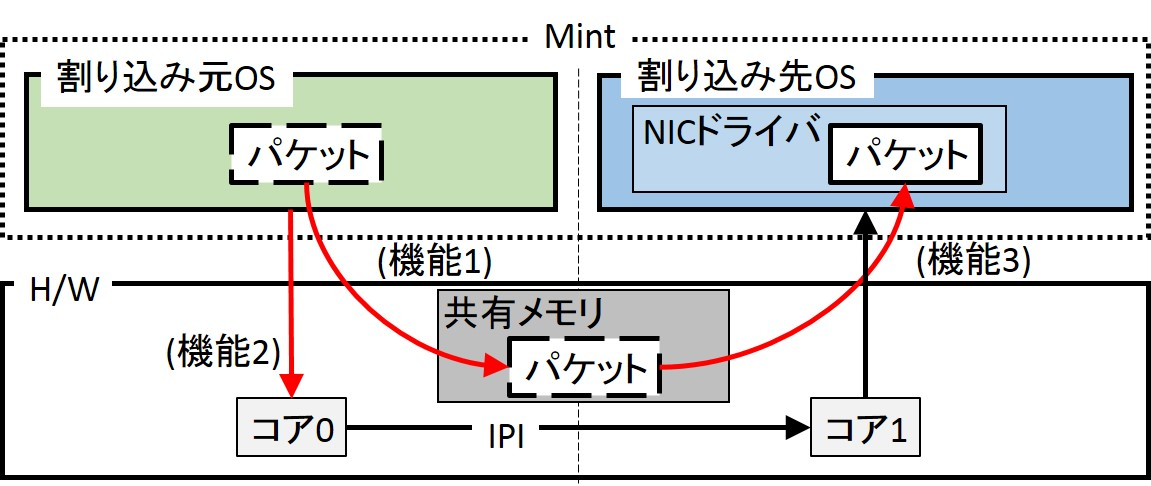
\includegraphics[height=5.0cm]{./fig1.jpg}
\caption{最終目標}
\label{fig1}
\end{center}
\end{figure}

\section{実験}
本実験について図2に示し,以下で説明する.
主に3章における(機能3)について実験を行った.
本実験では割り込み先OSのNICドライバ内でメッセージを表示する割り込みハンドラを登録し,
IPIの受信を契機としてこれを動作させた.
今回の実験では共有メモリとパケットについては考慮していない.
本実験における機能を以下に示す.
\begin{itemize}
\item[(機能1)] コア0にIPI送信要求を出し,コア0からコア1へIPIを送信する.
\item[(機能2)] コア1がIPIを受信すると,カーネルの受信バッファにメッセージを格納する.
\end{itemize}






\begin{figure}[t]
\begin{center}
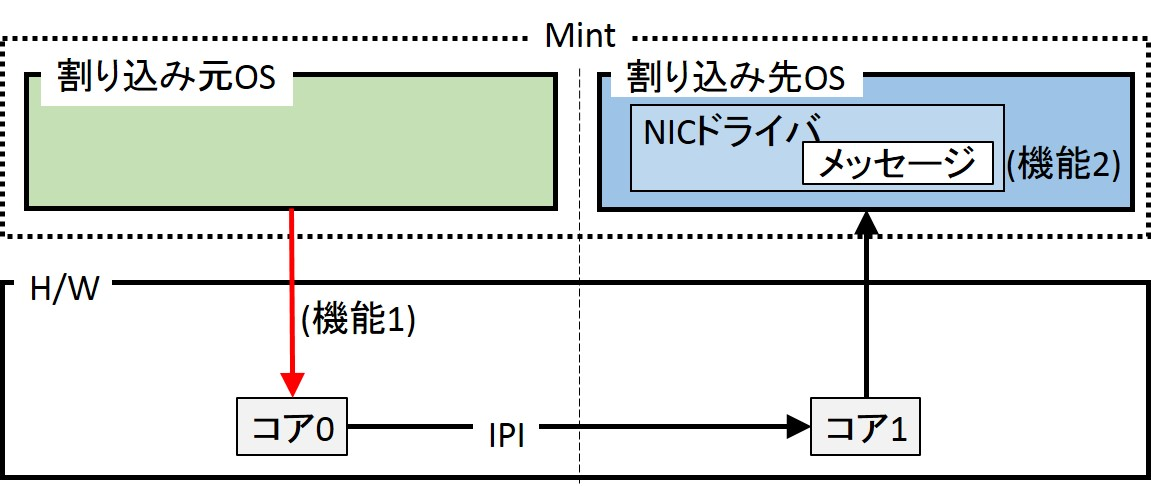
\includegraphics[height=5.0cm]{./fig2.jpg}
\caption{本実験における流れ}
\label{fig2}
\end{center}
\end{figure}



\section{割り込みハンドラの登録}
rtl8169\_open()内ではNICドライバの割り込みハンドラであるrtl8169\_interrupt()が登録されている.
この関数内で,IPIを受信するとメッセージを表示する割り込みハンドラを追加登録した.
割り込みハンドラの登録にはirq\_request()が使用されている.
この関数について以下に示す.
\begin{itemize}
\item [【形式】] static inline int \_\_must\_check int request\_irq(unsigned int irq, irq\_handler\_t handler, unsigned long flags,
 const char *name, void dev*)
\item [【引数】] unsigned int irq: IRQ番号\\
irq\_handler\_t handler: 登録する割り込みハンドラ\\
unsigned long flags: IRQの処理に関するフラグ\\
const char *name: /proc/interruptsに表示される名前\\
void dev*: デバイス
\item [【戻り値】] 成功: 0\\失敗: 0以外
\item [【機能】] irq\_desc構造体に割り込みハンドラを登録する.
\end{itemize}


\section{登録した割り込みハンドラ}
割り込みハンドラfujita\_ipi\_handler()を作成し,登録した.
これは「handler test」というメッセージを表示する割り込みハンドラである.
このハンドラを以下に示す.
\begin{itemize}
\item [【形式】] irqreturn\_t fujita\_ipi\_handler\_test(int irq, void *dev\_id)
\item [【引数】] int irq: 割り込みハンドラを登録するIRQ番号
void dev\_id*: デバイスID
\item [【戻り値】] var配列のcpu要素
\item [【機能】] printk()を呼び出し,カーネルのメッセージバッファに「handler test」と表示する.
\end{itemize}

\section{IPIによる呼び出し}
割り込み元OSの占有するコア0から割り込み先OSの占有するコア1へIPIを送信し,
fujita\_ipi\_handlerを動作させた.
IPIを送信すると割り込み先OSのカーネルの受信バッファに「handler test」というメッセージが格納されていたため,
割り込みハンドラが正しく登録され,動作していることを確認した.
IPIの送信は山本凌平さんの作成したシステムコールを登録し,使用した.
このシステムコールを以下に示す.
\begin{itemize}
\item [【形式】] asmlinkage void send\_yamamoto\_ipi(int core\_id, int vector, int n, int interval)
\item [【引数】] int core\_id:IPI送信先のコアID\\int vector:ベクタ番号\\int n:IPI送信回数\\int interval:IPI送信間隔
\item [【戻り値】] なし
\item [【機能】] core\_idのコアIDを持つコアへベクタ番号vectorの割り込みハンドラを実行させるIPIをn回連続で送信する.この際,IPIの送信間隔はintervalである.
\end{itemize}


\section{おわりに}
NICドライバのソースコード内で割り込みハンドラを登録し,IPIによってこれを動作できることを
確認した.
今後は,rtl8169の割り込みハンドラであるrtl8169\_interruptをIPIによって動作できるように
改変したものを新規に割り込みハンドラとして登録し,パケットを共有メモリから取得できるようにすることで3章における(機能3)を実装する.
また,共有メモリに擬似的なNICドライバの受信バッファを作成し,3章における(機能1)を実装する.
\end{document}


